% Compile with XeLaTeX
\documentclass[12pt,a4paper]{article}

\usepackage[a4paper,margin=2.2cm]{geometry}
\usepackage{fontspec}
\usepackage{amsmath,amssymb}
\usepackage{array,booktabs,longtable,multirow}
\usepackage[dvipsnames]{xcolor}
\usepackage{hyperref}
\usepackage{enumitem}
\usepackage{listings}
\usepackage[most]{tcolorbox}
\usepackage{tikz}
\usetikzlibrary{arrows.meta,positioning,fit,shapes.geometric}

\setmainfont{Times New Roman}
\setmonofont{Consolas}
\hypersetup{colorlinks=true,linkcolor=blue,urlcolor=blue}
\setlength{\parindent}{0pt}
\setlength{\parskip}{0.5em}

\lstdefinestyle{svstyle}{
  basicstyle=\ttfamily\small,
  keywordstyle=\color{blue!70!black}\bfseries,
  commentstyle=\color{gray!80!black},
  stringstyle=\color{BrickRed},
  showstringspaces=false,
  breaklines=true,
  frame=single,
  rulecolor=\color{black!20},
  columns=fullflexible
}

\title{Tai lieu doc hieu va trinh bay do an\\[4pt]
\Large Giai thich duong tin hieu Detection trong Intelli-Safe SoC}
\author{Soan tu RTL hien tai cua du an In\_SOC}
\date{\today}

\begin{document}
\maketitle
\tableofcontents
\newpage

\section{Muc tieu cua tai lieu}
Tai lieu nay duoc viet de phuc vu hai muc tieu:
\begin{enumerate}[label=\arabic*.]
    \item Giup sinh vien doc va hieu dung luong tin hieu trong do an, dac biet la duong \textbf{SPI/ADC $\rightarrow$ DSP detection $\rightarrow$ IRQ $\rightarrow$ CPU/GPIO relay}.
    \item Giup trinh bay voi giao vien huong dan bang ngon ngu ky thuat, nhung van de theo doi va doi chieu truc tiep voi RTL that cua du an.
\end{enumerate}

Pham vi tai lieu tap trung vao:
\begin{itemize}
    \item Top-level \texttt{top\_soc}
    \item Khoi \texttt{apb\_spi\_adc\_bridge}
    \item Khoi \texttt{logic\_bist}
    \item Khoi \texttt{dsp\_arc\_detect}
    \item Co che \texttt{inout} cua \texttt{gpio\_pin\_io}
\end{itemize}

\section{Tong quan kien truc can nho truoc khi doc}
Ve mat chuc nang, du an co the duoc hieu nhu sau:
\begin{center}
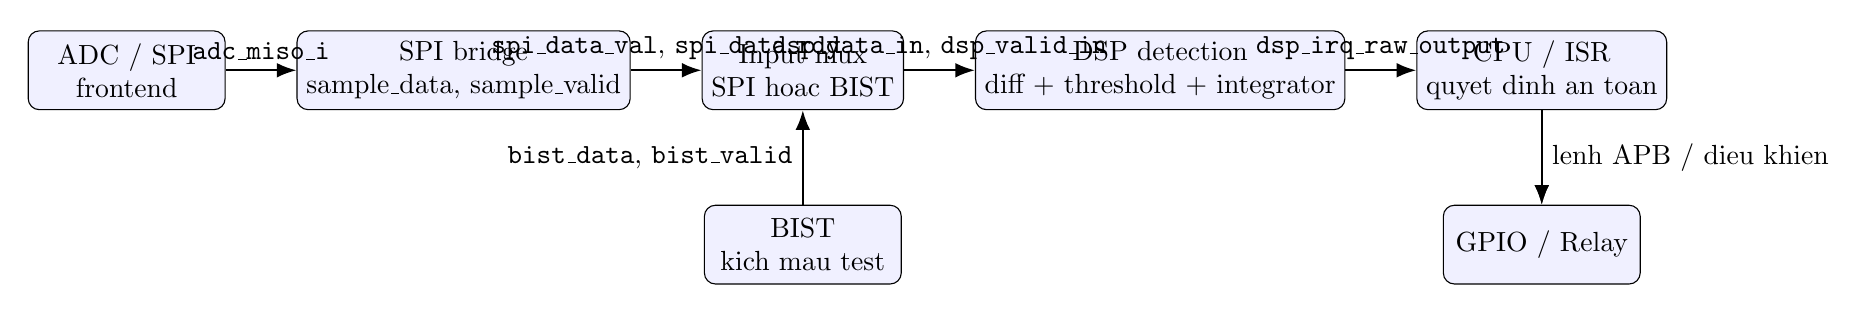
\begin{tikzpicture}[
    node distance=12mm and 9mm,
    block/.style={draw, rounded corners, minimum width=2.5cm, minimum height=1cm, fill=blue!6, align=center},
    line/.style={-{Latex[length=2.5mm]}, thick}
]
\node[block] (adc) {ADC / SPI\\frontend};
\node[block, right=of adc] (spi) {SPI bridge\\sample\_data, sample\_valid};
\node[block, right=of spi] (mux) {Input mux\\SPI hoac BIST};
\node[block, right=of mux] (dsp) {DSP detection\\diff + threshold + integrator};
\node[block, right=of dsp] (cpu) {CPU / ISR\\quyet dinh an toan};
\node[block, below=of mux] (bist) {BIST\\kich mau test};
\node[block, below=of cpu] (gpio) {GPIO / Relay};

\draw[line] (adc) -- node[above]{\texttt{adc\_miso\_i}} (spi);
\draw[line] (spi) -- node[above]{\texttt{spi\_data\_val}, \texttt{spi\_data\_rdy}} (mux);
\draw[line] (bist) -- node[left]{\texttt{bist\_data}, \texttt{bist\_valid}} (mux);
\draw[line] (mux) -- node[above]{\texttt{dsp\_data\_in}, \texttt{dsp\_valid\_in}} (dsp);
\draw[line] (dsp) -- node[above]{\texttt{dsp\_irq\_raw\_output}} (cpu);
\draw[line] (cpu) -- node[right]{lenh APB / dieu khien} (gpio);
\draw[line] (cpu) -- (gpio);
\end{tikzpicture}
\end{center}

Y chinh can nho:
\begin{itemize}
    \item \textbf{DSP khong nhan truc tiep ADC top-level.} No nhan du lieu da duoc tien xu ly thanh cap \texttt{dsp\_data\_in} va \texttt{dsp\_valid\_in} tai \texttt{top\_soc}.
    \item \textbf{BIST co the chiem duong vao DSP.} Khi BIST dang chay, du lieu that tu SPI bi thay the bang mau test.
    \item \textbf{IRQ quan trong tu DSP bi mask trong luc BIST chay.} Dieu nay tranh BIST gay ngat gia len CPU.
\end{itemize}

\section{Dinh nghia chinh xac cac cong top-level}
Cac cong top-level trong \texttt{top\_soc} co y nghia sau:

\begin{longtable}{>{\ttfamily}p{3cm} p{1.8cm} p{9.2cm}}
\toprule
\textnormal{Ten cong} & \textnormal{Loai} & \textnormal{Y nghia} \\
\midrule
\endhead
\texttt{clk\_i} & input & Clock he thong, tan so danh dinh 50 MHz. Day la clock chung cho CPU, SPI bridge, DSP, timer, watchdog, BIST. \\
\texttt{rst\_ni\_async} & input & Reset ngoai, active-low. Tinh hieu nay duoc ket hop voi watchdog reset de tao \texttt{combined\_rst\_n}, sau do duoc dong bo thanh \texttt{rst\_no}. \\
\texttt{adc\_miso\_i} & input & Du lieu noi tiep di tu ADC vao SoC. Khoi SPI bridge doc tin hieu nay de tao ra sample song song 16-bit. \\
\texttt{adc\_mosi\_o} & output & Du lieu tu SoC gui nguoc lai ADC. Trong cau hinh hien tai bridge cho phep ton tai cong nay de mo rong sau nay. \\
\texttt{adc\_sclk\_o} & output & Xung clock SPI do bridge tao ra. \\
\texttt{adc\_csn\_o} & output & Chip-select cho ADC, active-low. \\
\texttt{uart\_tx\_o} & output & Tin hieu truyen UART tu SoC ra ngoai. \\
\texttt{uart\_rx\_i} & input & Tin hieu nhan UART tu ngoai vao SoC. \\
\texttt{gpio\_pin\_io[3:0]} & inout & Cum chan GPIO hai chieu. Trong do bit 0 dung cho relay an toan, cac bit con lai co the la chi bao trang thai va tin hieu phu. \\
\bottomrule
\end{longtable}

\section{Phan biet \texttt{input}, \texttt{output}, \texttt{inout}}
\subsection{Khi nao la mux input?}
Neu mot tin hieu duoc tao bang cau truc kiem tra dieu kien roi chon mot trong hai nguon, do la \textbf{mux}. Vi du trong \texttt{top\_soc}:
\begin{lstlisting}[style=svstyle]
assign dsp_data_in  = bist_active_mode ? bist_data  : spi_data_val;
assign dsp_valid_in = bist_active_mode ? bist_valid : spi_data_rdy;
\end{lstlisting}

Dieu nay co nghia la:
\begin{itemize}
    \item Neu \texttt{bist\_active\_mode = 1} thi DSP nhan du lieu test tu BIST.
    \item Neu \texttt{bist\_active\_mode = 0} thi DSP nhan du lieu that tu SPI bridge.
\end{itemize}

\subsection{Khi nao la \texttt{inout}?}
\texttt{inout} khong phai la mux. \texttt{inout} la mot chan co the:
\begin{itemize}
    \item duoc \textbf{drive} ra ngoai khi direction cho phep,
    \item hoac duoc \textbf{tha noi troi} (high impedance, \texttt{'z}) de ngoai vi hoac thiet bi khac drive vao.
\end{itemize}

Trong \texttt{top\_soc}, co che \texttt{inout} cua GPIO duoc viet nhu sau:
\begin{lstlisting}[style=svstyle]
assign gpio_pin_io[0]   = (!rst_no) ? 1'b0 :
                          (gpio_dir_wire[0] ? gpio_out_wire[0] : 1'bz);
assign gpio_pin_io[3:1] = gpio_dir_wire[3:1] ? gpio_out_wire[3:1] : 3'bz;
\end{lstlisting}

Y nghia:
\begin{itemize}
    \item \texttt{gpio\_dir\_wire[i] = 1}: SoC chu dong la nguoi xuat du lieu ra chan do.
    \item \texttt{gpio\_dir\_wire[i] = 0}: SoC khong lai chan do, chan o trang thai \texttt{Z}.
    \item Bit 0 con duoc ep ve 0 trong luc reset de giu relay o trang thai an toan.
\end{itemize}

\section{Duong vao chinh xac cua khoi detection}
Khoi detection trong du an la \texttt{dsp\_arc\_detect}. Cac cong cua no duoc noi tai \texttt{top\_soc} nhu sau:
\begin{lstlisting}[style=svstyle]
dsp_arc_detect u_dsp (
    .clk_i       (clk_i),
    .rst_ni      (rst_no),
    .adc_data_i  (dsp_data_in),
    .adc_valid_i (dsp_valid_in),
    .apb_slv     (apb_dsp_if),
    .irq_arc_o   (dsp_irq_raw_output)
);
\end{lstlisting}

\subsection{Bang dinh nghia input/output cua khoi DSP}
\begin{longtable}{>{\ttfamily}p{3cm} p{1.5cm} p{9.5cm}}
\toprule
\textnormal{Tin hieu} & \textnormal{Loai} & \textnormal{Dinh nghia chinh xac} \\
\midrule
\endhead
\texttt{clk\_i} & input & Clock cua khối DSP. O project hien tai no duoc noi truc tiep voi \texttt{clk\_i} cua toan he thong. \\
\texttt{rst\_ni} & input & Reset dong bo sau bo \texttt{rstgen}. Day khong phai reset ngoai truc tiep, ma la \texttt{rst\_no}. \\
\texttt{adc\_data\_i[15:0]} & input & Mau du lieu 16-bit dua vao thuat toan detection. Tin hieu nay thuc chat la \texttt{dsp\_data\_in}. \\
\texttt{adc\_valid\_i} & input & Xung bao mau hop le di kem voi \texttt{adc\_data\_i}. Tin hieu nay thuc chat la \texttt{dsp\_valid\_in}. \\
\texttt{apb\_slv} & interface input & Kenh APB de CPU cau hinh threshold, limit, decay, attack va doc telemetry cua DSP. \\
\texttt{irq\_arc\_o} & output & Tin hieu bao phat hien ho quang tu DSP. O top-level no duoc dat ten trung gian la \texttt{dsp\_irq\_raw\_output}. \\
\bottomrule
\end{longtable}

\subsection{Nguon thuc su cua \texttt{adc\_data\_i} va \texttt{adc\_valid\_i}}
Day la phan rat quan trong khi trinh bay:
\begin{align*}
\texttt{dsp\_data\_in} &= \begin{cases}
\texttt{bist\_data} & \text{neu } \texttt{bist\_active\_mode}=1 \\
\texttt{spi\_data\_val} & \text{neu } \texttt{bist\_active\_mode}=0
\end{cases} \\
\texttt{dsp\_valid\_in} &= \begin{cases}
\texttt{bist\_valid} & \text{neu } \texttt{bist\_active\_mode}=1 \\
\texttt{spi\_data\_rdy} & \text{neu } \texttt{bist\_active\_mode}=0
\end{cases}
\end{align*}

Noi cach khac, \textbf{input vao khoi detection khong duoc chon truc tiep tu cong top-level, ma duoc chon tai top-level bang mot bo mux noi bo}.

\section{Vai tro cua SPI bridge trong duong detection}
Khoi \texttt{apb\_spi\_adc\_bridge} dong vai tro chuyen doi du lieu SPI thanh sample song song phuc vu DSP.

Cac output can nho cua bridge:
\begin{itemize}
    \item \texttt{sample\_data\_o} $\rightarrow$ duoc noi thanh \texttt{spi\_data\_val}
    \item \texttt{sample\_valid\_o} $\rightarrow$ duoc noi thanh \texttt{spi\_data\_rdy}
    \item \texttt{busy\_o}, \texttt{frame\_active\_o}, \texttt{overrun\_o} $\rightarrow$ cac co trang thai/chan doan
\end{itemize}

Snippet can nho:
\begin{lstlisting}[style=svstyle]
.sample_data_o  (spi_data_val),
.sample_valid_o (spi_data_rdy),
.busy_o         (spi_busy),
.frame_active_o (spi_frame_active),
.overrun_o      (spi_overrun)
\end{lstlisting}

Khi trinh bay voi giao vien, ban co the noi ngắn gọn:
\begin{quote}
``Khoi SPI bridge nhan bit serial tu ADC qua \texttt{adc\_miso\_i}, dong goi thanh sample 16-bit, sau do phat xung \texttt{sample\_valid} de thong bao cho DSP biet rang da co mau hop le moi.''
\end{quote}

\section{Vai tro cua BIST trong duong detection}
Khoi \texttt{logic\_bist} co ba output chinh lien quan truc tiep den duong detection:
\begin{itemize}
    \item \texttt{bist\_data\_o} $\rightarrow$ noi thanh \texttt{bist\_data}
    \item \texttt{bist\_valid\_o} $\rightarrow$ noi thanh \texttt{bist\_valid}
    \item \texttt{bist\_active\_o} $\rightarrow$ noi thanh \texttt{bist\_active\_mode}
\end{itemize}

Y nghia he thong:
\begin{itemize}
    \item BIST co the cho DSP an mau gia lap de tu kiem tra.
    \item Trong luc BIST dang chay, du lieu that tu ADC/SPI khong duoc dua vao DSP.
    \item CPU cung khong nen nhan IRQ nguy hiem gia trong luc nay, nen top-level mask duong \texttt{irq\_arc\_critical}.
\end{itemize}

Snippet quan trong:
\begin{lstlisting}[style=svstyle]
assign irq_arc_critical = bist_active_mode ? 1'b0 : dsp_irq_raw_output;
\end{lstlisting}

\section{Nguyen ly hoat dong noi bo cua khoi DSP detection}
DSP hien tai la mot detector don gian theo kien truc:
\begin{center}
\textbf{Sai khac giua hai mau lien tiep} $\rightarrow$ \textbf{so sanh threshold} $\rightarrow$ \textbf{leaky integrator} $\rightarrow$ \textbf{IRQ}
\end{center}

\subsection{Buoc 1: Tao sai khac giua hai mau lien tiep}
\begin{lstlisting}[style=svstyle]
assign diff_raw_comb = signed(adc_data_i) - signed(sample_prev_q);
assign diff_abs_comb = abs_diff(diff_raw_comb);
\end{lstlisting}

\textbf{Y nghia:} DSP khong quan tam gia tri tuyet doi cua mot mau don le, ma quan tam do thay doi giua hai mau lien tiep.

\subsection{Buoc 2: Kiem tra co phai spike hay khong}
\begin{lstlisting}[style=svstyle]
assign is_spike_detected = sample_pair_valid && adc_valid_i &&
                           (diff_abs_comb > reg_diff_threshold);
\end{lstlisting}

Ba dieu kien phai dong thoi dung:
\begin{enumerate}[label=\arabic*.]
    \item Da co du it nhat mot cap mau hop le (\texttt{sample\_pair\_valid = 1})
    \item Hien tai dang co mau moi (\texttt{adc\_valid\_i = 1})
    \item Sai khac vuot nguong \texttt{reg\_diff\_threshold}
\end{enumerate}

\textbf{Diem cai tien Phase 1:} Dieu kien \texttt{sample\_pair\_valid} tranh loi cu trong do mau thu hai bi so voi 0 thay vi so voi mau thu nhat.

\subsection{Buoc 3: Leaky integrator}
Neu co spike, DSP cong them \texttt{attack}. Neu khong co spike, DSP giam dan theo \texttt{decay}.
\begin{align*}
\texttt{integrator\_after\_attack} &= \min(\texttt{integrator} + \texttt{attack}, \texttt{limit}) \\
\texttt{integrator\_after\_decay} &= \max(\texttt{integrator} - \texttt{decay}, 0)
\end{align*}

Y nghia vat ly:
\begin{itemize}
    \item Nhieu spike lien tiep se lam ``thung tich luy'' day len dan.
    \item Nhieu xung don le hoac nhiu ngan se bi ``ro ri'' xuong va khong du suc gay bao dong.
\end{itemize}

\subsection{Buoc 4: Ra quyet dinh}
Khi \texttt{integrator} dat den \texttt{reg\_int\_limit}, DSP set:
\begin{itemize}
    \item \texttt{irq\_arc\_o = 1}
    \item \texttt{fire\_latched = 1}
    \item \texttt{reg\_status = FIRE}
\end{itemize}

\section{Cac thanh ghi APB quan trong cua DSP}
Khoi DSP duoc map tai base address:\
\texttt{DSP\_BASE\_ADDR = 0x0000\_1000}

\begin{longtable}{>{\ttfamily}p{2.3cm} >{\ttfamily}p{2cm} p{9.5cm}}
\toprule
\textnormal{Dia chi} & \textnormal{Ten} & \textnormal{Y nghia} \\
\midrule
\endhead
\texttt{0x1000} & STATUS & Trang thai tong hop: \texttt{reg\_status}, \texttt{irq\_arc\_o}, \texttt{fire\_latched}, \texttt{sample\_pair\_valid}. \\
\texttt{0x1004} & DIFF\_THRESH & Nguong de quyet dinh mot bien doi co du lon de duoc coi la spike hay khong. \\
\texttt{0x1008} & INT\_LIMIT & Gioi han cua leaky integrator. Vuot muc nay thi phat IRQ. \\
\texttt{0x100C} & DECAY\_RATE & Toc do giam cua integrator khi khong co spike. \\
\texttt{0x1010} & ATTACK\_RATE & Toc do tang cua integrator khi co spike. \\
\texttt{0x1014} & CUR\_DIFF & Gia tri sai khac hien tai giua hai mau lien tiep. \\
\texttt{0x1018} & CUR\_INT & Gia tri integrator hien tai. \\
\texttt{0x101C} & PEAK\_DIFF & Sai khac lon nhat da quan sat. \\
\texttt{0x1020} & PEAK\_INT & Gia tri integrator lon nhat da dat duoc. \\
\texttt{0x1024} & EVENT\_COUNT & So lan detector da fire. \\
\texttt{0x1028} & CLEAR & Xoa co sticky, xoa peak telemetry, xoa event counter theo bit dieu khien. \\
\bottomrule
\end{longtable}

\section{Giai thich co che \texttt{gpio\_pin\_io} cho de trinh bay}
Phan nay rat de duoc hoi boi giao vien vi tu \texttt{inout} thuong gay nham lan.

\subsection{Bit 0: relay an toan}
\begin{itemize}
    \item \texttt{gpio\_pin\_io[0]} duoc dung de dieu khien relay.
    \item Trong luc reset, bit nay bi ep ve 0 de giu he thong an toan.
    \item Sau reset, neu \texttt{gpio\_dir\_wire[0] = 1} thi SoC moi duoc quyen lai relay bang \texttt{gpio\_out\_wire[0]}.
    \item Neu \texttt{gpio\_dir\_wire[0] = 0} thi chan o trang thai high impedance.
\end{itemize}

\subsection{Bits 3:1}
\begin{itemize}
    \item Co the dung de hien thi trang thai, doc input ngoai, hoac mo rong chuc nang.
    \item Gia tri doc vao khoi GPIO duoc lay bang:
\begin{lstlisting}[style=svstyle]
assign gpio_in_wire[3:1] = gpio_pin_io[3:1];
\end{lstlisting}
\end{itemize}

\textbf{Ket luan can noi voi giao vien:}
\begin{quote}
``Trong du an nay, \texttt{inout} duoc thuc hien bang co che direction bit va tri-state. Day la mot co che khac ban chat voi viec chon nguon input cua DSP, vi input DSP duoc chon bang mux noi bo, con \texttt{inout} GPIO duoc quyet dinh bang quyen drive hay tha high-impedance.''
\end{quote}

\section{Nhung cau noi goi y khi trinh bay voi giao vien}
Ban co the trinh bay ngan gon theo trinh tu sau:

\begin{tcolorbox}[colback=blue!3,colframe=blue!40!black,title=Goi y cach noi]
\begin{enumerate}[label=\arabic*.]
    \item ``Top-level cua em nhan du lieu serial tu ADC qua \texttt{adc\_miso\_i}.''
    \item ``Khoi SPI bridge bien doi luong serial do thanh sample song song 16-bit va phat xung \texttt{sample\_valid}.''
    \item ``Truoc khi vao khoi detection, top-level co mot bo mux de chon giua du lieu that tu SPI va du lieu test tu BIST.''
    \item ``Khoi DSP detection khong nhan truc tiep cong top-level, ma nhan hai tin hieu trung gian la \texttt{dsp\_data\_in} va \texttt{dsp\_valid\_in}.''
    \item ``Ben trong DSP, em dung sai khac giua hai mau lien tiep, so sanh voi threshold, roi dua vao leaky integrator de loc nhiu va phat hien ho quang lien tuc.''
    \item ``Neu integrator dat gioi han, DSP phat IRQ sang CPU; CPU sau do xu ly an toan va dieu khien relay qua GPIO.''
\end{enumerate}
\end{tcolorbox}

\section{Ba diem de giao vien de hoi va cach tra loi}
\subsection*{Cau hoi 1: Tai sao khong dua ADC vao DSP truc tiep?}
Tra loi: Vi du an can mot lop giao tiep SPI de thu bit serial tu ADC, tao sample 16-bit, dong thoi de mo rong APB control/status cho firmware.

\subsection*{Cau hoi 2: Tai sao BIST co the chen vao duong DSP?}
Tra loi: De tu kiem tra khong phu thuoc vao ADC that. BIST tao mau test co chu dich, dua vao cung duong ma DSP dung binh thuong.

\subsection*{Cau hoi 3: Tai sao phai mask IRQ khi BIST chay?}
Tra loi: Vi trong luc test, BIST co the co y tao ra mau giong su kien loi. Neu khong mask, CPU co the hieu nham day la ho quang that.

\section{Ket luan ky thuat ngan gon}
Tu goc nhin he thong, duong detection cua do an hien tai duoc hinh dung nhu sau:
\begin{center}
\texttt{adc\_miso\_i} $\rightarrow$ \texttt{SPI bridge} $\rightarrow$ \texttt{spi\_data\_val / spi\_data\_rdy}
$\rightarrow$ \texttt{mux voi BIST} $\rightarrow$ \texttt{dsp\_data\_in / dsp\_valid\_in}
$\rightarrow$ \texttt{dsp\_arc\_detect} $\rightarrow$ \texttt{dsp\_irq\_raw\_output}
$\rightarrow$ \texttt{CPU / GPIO relay}
\end{center}

Diem quan trong nhat de nho khi trinh bay la:
\begin{itemize}
    \item Input cua khoi detection duoc chon bang mux trong \texttt{top\_soc}.
    \item \texttt{inout} GPIO duoc quyet dinh bang direction bit va tri-state.
    \item DSP detection hien tai dung kien truc \textit{difference + static threshold + leaky integrator}.
    \item BIST co the chiem duong vao DSP, va top-level chu dong mask IRQ de tranh false alarm.
\end{itemize}

\section*{Ghi chu su dung}
Ban nen compile file nay bang \textbf{XeLaTeX}. Neu can, co the doi ten file thanh mot ten de nho hon nhu \texttt{dsp\_detection\_guide.tex} ma khong anh huong noi dung.

\end{document}
